\documentclass[12pt]{article}

\usepackage{sbc-template}

\usepackage{graphicx,url}

\usepackage[brazil]{babel}   
%\usepackage[latin1]{inputenc}  
\usepackage[utf8]{inputenc}  
% UTF-8 encoding is recommended by ShareLaTex

     
\sloppy

\title{Review: Handover Implementation in a 5G SDN-based Mobile Network Architecture}

\author{Antônio O. Junior\inst{1}, Cleverson V. Nahum\inst{1}, Felipe H. B. Bastos\inst{1}, Jamelly F. Ferreira\inst{1}, \\João C. Belmiro\inst{1} }


\address{Faculdade de Engenharia da Computação e Telecomunicações \\-- Universidade Federal do Pará
  (UFPA)\\
  Caixa Postal 479 -- 66.075-110 -- Belém -- PA -- Brazil
  \email{\{antonio,jamelly.ferreira,felipe,joao\}@itec.ufpa.br, cleversonahum@ufpa.br}
}

\begin{document} 

\maketitle

\begin{abstract}
  This meta-paper describes the style to be used in articles and short papers
  for SBC conferences. For papers in English, you should add just an abstract
  while for the papers in Portuguese, we also ask for an abstract in
  Portuguese (``resumo''). In both cases, abstracts should not have more than
  10 lines and must be in the first page of the paper.
\end{abstract}
     
\begin{resumo} 
  Este meta-artigo descreve o estilo a ser usado na confecção de artigos e
  resumos de artigos para publicação nos anais das conferências organizadas
  pela SBC. É solicitada a escrita de resumo e abstract apenas para os artigos
  escritos em português. Artigos em inglês deverão apresentar apenas abstract.
  Nos dois casos, o autor deve tomar cuidado para que o resumo (e o abstract)
  não ultrapassem 10 linhas cada, sendo que ambos devem estar na primeira
  página do artigo.
\end{resumo}


\section{Introduction}
With the rapid expansion of the mobile environment there is a need to improve Internet connectivity so that the user has a better experience. The 5G technology comes with the proposal to offer greater bandwidth for mobile devices, the main motivations for the emergence of 5G are: According to estimates, seventy per cent of the world's population will use mobile devices, Emergence of new enterprises in which they demanded a higher quality of service, as, information of all things, deep learning of the machine, support things, digital assistants keeping conversation with clients, augmented reality, 3D printing, intra body networks. The requirements for implementing 5G networks are the flexibility and scalability of the network, and a less costly processing and memory demand beyond greater energy efficiency than its predecessor. In order to improve 5G, it is necessary to use new network architectures such as Software Defined Networking (SDN) and Network Functions Virtualization (NFV).

The most successful initiative in this regard was undoubtedly the interface and the Openflow protocol. With Openflow, the routing elements provide a simple programming interface, which allows them to extend access and control of the query table used by the hardware to determine the next step of each received packet. In this way, the routing continues to be efficient, since the query to the routing table remains a task of the hardware, but the decision on how each package should be processed can be transferred to a level superior, where different features can be added. This structure allows the network to be extensively controlled through, expressed in software. This new paradigm was called Software Defined Networks (SDN). NFV is the support for defining services such as VPN, WAN, intrusion detection, firewall and so on. It is about virtualizing functions that were previously performed by physical devices. Now they can be defined by software, and can be adapted to various types of network equipment and standard servers in the market, thus becoming revenue generating services.

Both the network and the virtualization of its functions are related. NFV is complementary to SDN, but does not depend on it, or contrariwise. NFV can be implemented without SDN. NFV can be implemented without an SDN; however, the two concepts and solutions are combined for more efficiency and mutually beneficial. But, in reality, SDN makes the NFV more attractive because a software-defined network contributes to the automation of its infrastructure, which allows policy-based decisions to orchestrate network traffic. And respectively, the virtualization of network functions acts directly on the services ensures their capacity, aligned with the virtualized elements.

Conferences that publish just abstracts ask for \textbf{one}-page texts.

\section{Background SDN and NFV} \label{sec:sdn}
\subsection{SDN}

The SDN (Software-Defined Networking) is a recently concept of network, nowadays the most part of the networks has a distributed control in the their elements. So, with the growth of the multimedia and the increases of flows of data traffic in the world, it emerged necessity to have more control over the network and more mobility in the chooses, the networks need to be more flexible. With this need the SDN was thought to solve some problems in the actual architecture.

The main of SDN is split the data plane (data flow) of control plane (control flow) and centralized all the control of the network in a unique place named Controller. In the SDN, it has a division between APPs, control plane and data plane, it is possible to seen in (Figure 1). The APPs are applications with functions related to security, network management and others, they are responsible to make security and other needs of the network, in the traditional architecture this responsible is distributed in the elements of network, how SDN has more informations about the network, it became more easy to make decisions about the flow paths, to solve congestions and other problems faced in networks.

The control plane is represented by the Controllers, it is responsible to control the switches OpenFlow in according with algorithms and configurations established in APPs. The communication between Controllers and APPs is done through northbound interface. With the Controllers is possible to set all the connections of the switch through software. The OpenFlow switch quoted is a special switch made for to work with SDN networks.

The data plane is represented by the switches, OpenFlow switches is the principal, The communication between Controllers and switches is done through southbound interface. The OpenFlow switches is more simple than traditional switches and its communication and iteration is made through a API. In the traditional switches we have a proprietor systems for each one, it became more complex to implement a network because the systems is much specifically. With the switches OpenFlow the work of switches is more simple and it can be more flexible, because now all the connections can be defined in the software, moreover, it has more freedom to make changes in its, because of the iteration level is higher than traditional switches.

\begin{figure}[ht]
\centering
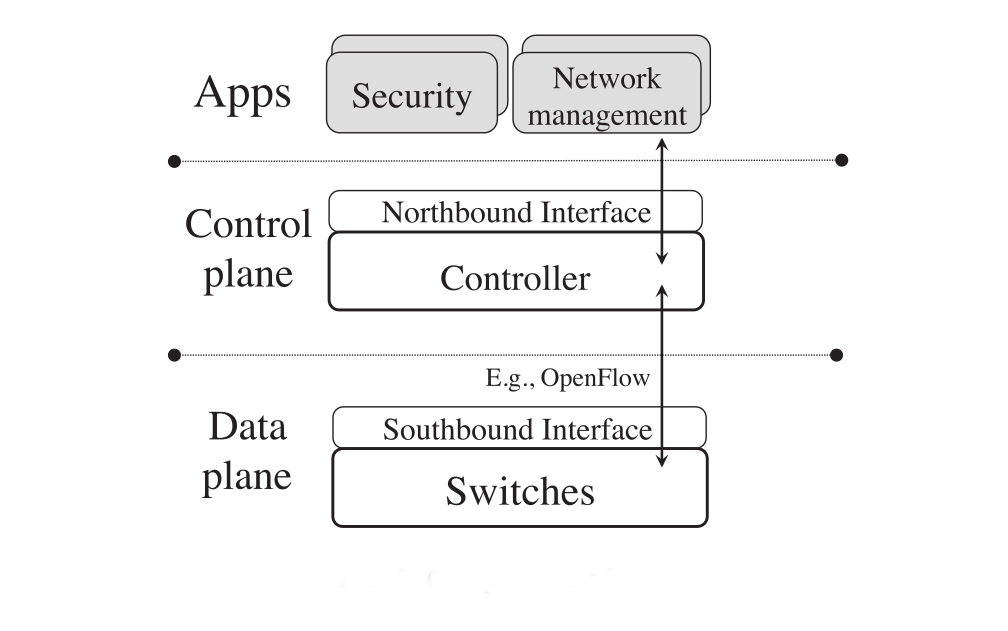
\includegraphics[width=.7\textwidth]{figure1.png}
\caption{Components of SDN}
\label{figure1}
\end{figure}

In the actual architecture, it has the data plane and control plane distributed on the routers, servers, clients ans other elements of the network, with this all the control of network became more complex and hard to manage. The SDN proposed a different way of see the network, it allow to centralize the control of network in a place, with is, it is possible to see all the nodes and connections of the network and to know about everything that occurs, thereby it is possible to do the better actions for to improve the network performance. The picture in (Figure 2) shows a illustrations of the difference between the networks in a traditional architecture, in a hybrid and using SDN. In a traditional networking, there is the data plane and control plane in all the components of the network, it is distributed. In hybrid networking there is a controller over the traditional networking for to control the switches and elements of the network. In the SDN, there is a clear division between data plane and control plane, the switches has only the data planes and the controller has the control plane.

\begin{figure}[ht]
\centering
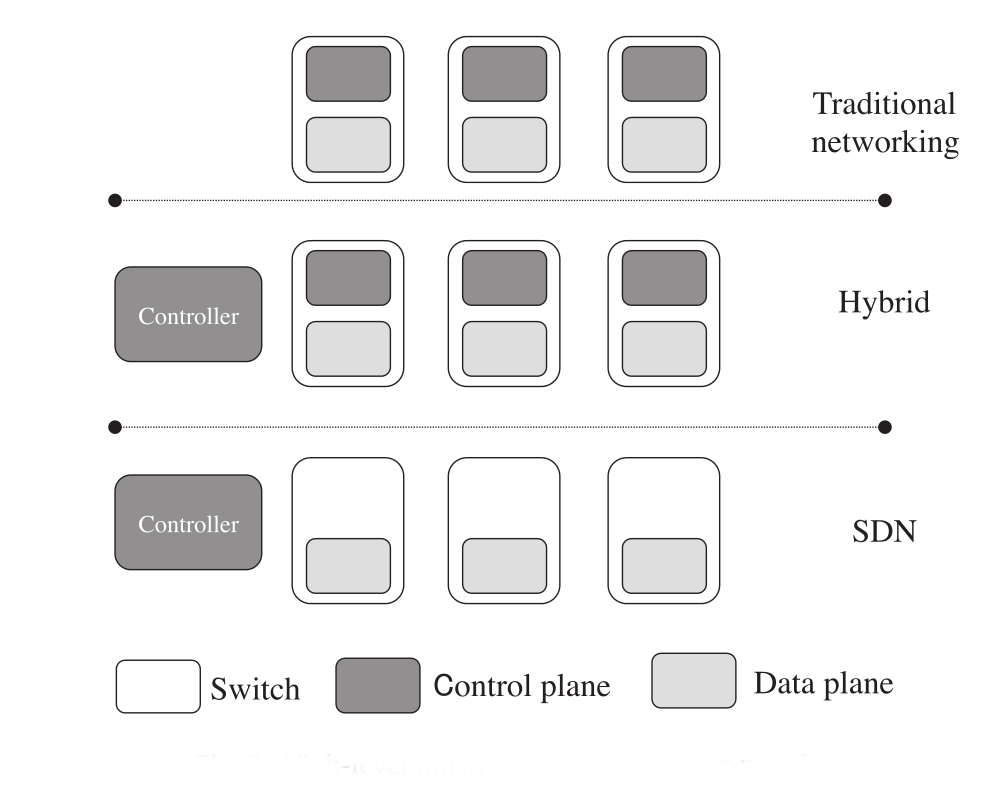
\includegraphics[width=.7\textwidth]{figure2.png}
\caption{High level illustration of networking paradigms}
\label{figure 2: High level illustration of networking paradigms}
\end{figure}

The OpenFlow is a communication protocol to provide access to switches. Sometimes the OpenFlow concept is confused with SDN, but the concepts are different, the OpenFlow work like a API to make communication between the control plane and data plane. In the picture in (Figure 3), it is a demonstration of the functions of OpenFlow. the OpenFlow controller works in user program to control the switches. In the OpenFlow switch there is a OpenFlow interface for to receive the commands of OpenFlow controller and after the changes are done in the forwarding tables and forwarding path.

\begin{figure}[ht]
\centering
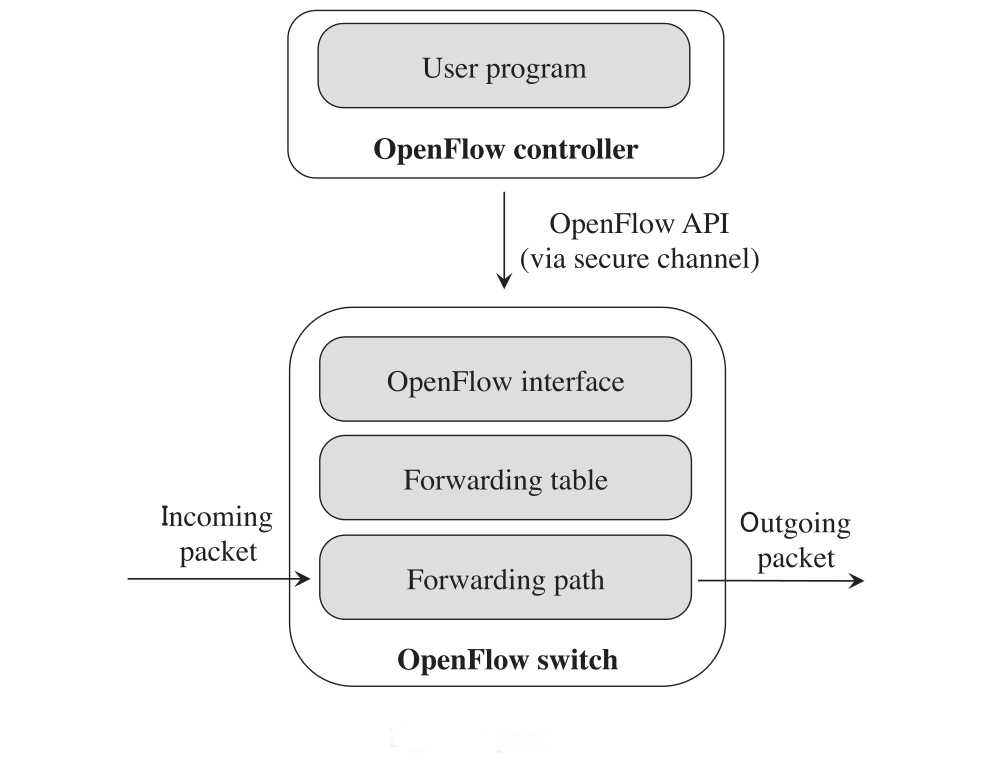
\includegraphics[width=.7\textwidth]{figure3.png}
\caption{OpenFlow}
\label{figure 3: OpenFlow}
\end{figure}


\subsection{NFV}

The NV (Network Virtualization) is a newly concept about networks using cloud computing and its resources. With the cloud computing, it became possible to set and use resources distributed in the network in according with the needs of the user. So, the resource is distributed and the control about this is remote and can be more precise and with higher performance than traditional architecture.

With the same idea of NV, emerged the concept o NFV (Network Function Virtualization), this concept is about to emulate into computational resources the elements of the network, like routers, firewalls and EPCs. This is very important to make networks more flexible, scalable and simple to manage.


\section{5G and Mobility}

The level of mobility is one of the key issues at the service level. In the 5G system, not all user equipments - UE requires continuous mobility and / or global reach. The level of mobility can be reduced to save network resources and reduce the complexity of the control. Some authors specifies a mobility level control (LoM) requirement in the connected UE state. The 5G system should enable operators to update the level of mobility support provided to a UE, for example, during the establishment of packet data connection.

Thee mobility level can be set in two modes: idle mode and connected mode. The mobility of the sleep mode can be defined for accessibility to the UE in idle mode. Mobility level in connected mode is set to handover level (HO), in this article we focuses on connected mode. To make more plain, handover is a process in telecommunications and mobile communications in which a cellular call or a data session is transferred from one base station to another without disconnecting the session. Cellular services are based on mobility and handover, allowing the user to be moved from one base station range to another or to be switched to the nearest base site for better performance.

In the LTE or 4G mobile system, the network always supports packet lossless mobility. This control overhead is not effective when the number of devices increases tremendously by 5G. In today's network services, most of the application, such as web browsing or chat, does not require seamless mobility. In addition, the application layer has its own mechanism for maintaining the level of application of service continuity. For these services, the network can handle mobility at a lower level than the current 4G system.

The level of mobility control is actively discussed in the 3GPP 5G architecture study. The mobility level (MdA) can be defined in two respects. The LoM of the Area (LoM-A) specifies the area where the UE can have mobility services - RAN, TA, EPC, LTE-5G and non-3GPP. LoM of Continuity (LoM-C) specifies the level of session continuity - uninterrupted mobility or interrupted mobility. To support the on-demand mobility requirement, the network must have an architecture to update (upgrade or downgrade) the LoM. To support the LoM update of the active session, the UE requests to change the LoM and the operator updates the LoM of the UE, if necessary. Updating the EU LoM-C and LoM-A requires monitoring the status of your application and its location. For example, the smart phone has the Internet messenger that supports the exchange of text messages and voice / video calls. When the user exchanges text messages, the UE does not need to support continuous mobility. But as soon as the UE invokes the voice / video call, continuous mobility is required. Depending on the state of your application, EU must request the LoM update for the network. Similar scenario for updating LoM-A can also be found.

Therefore, 5G network system must support multiple levels of mobility. For the connected mode mobility level, the HO level must be defined in two respects - continuity level and area level - and both aspects must be dynamically controllable - that is, the mobility level can be updated or degraded dynamically. The network architecture must be designed to satisfy the flexibility of control.

\section{Related Works}

In the context of future mobile networks , SDN and NFV concepts are present in almost all recent proposals in reason of the improvements on energy consumption,flexibility and cost. The difference of implementation approach, applied areas and the transition from legacy architectures to new paradigms are the main differences between them.

Some authors recomend a smooth and careful transition from the current networks to the future ones, as an example, adopting a 3-step approach trying to reduce the devaluation of the legacy network structure. In other hand, several authors are paying attemption to the mobility support in a SDN-based architecture through removing the  GTP-U protocol at UP, keeping the 3GPP unchanged and the use of legacy nodes or focusing in the mobility handling trying to find implementation challenges like session continuity. 

\subsection{Subsections}

The subsection titles must be in boldface, 12pt, flush left.

\section{System Architecture}

The architecture proposed in the work is a 5g mobile network for the AC(Acess Cloud) whith partial virtualization and SDN-based UP, this scenario is made by implementing the LTE CP as NFVs and running it in a logically centralized data center.

\begin{figure}[ht]
\centering
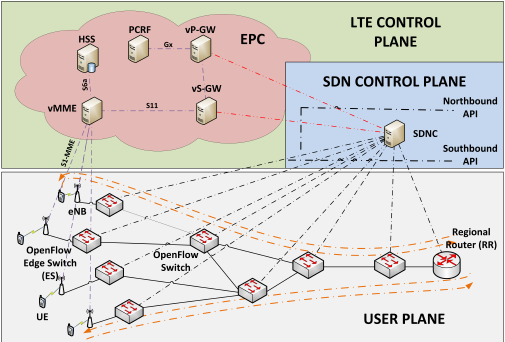
\includegraphics[width=.7\textwidth]{figurejamelly.png}
\caption{System Architecture}
\label{figure 4: System Architecture}
\end{figure}

In the work, the virtualized LTE control network design is based in a 1:N mapping architecture, so they are split in 3 components : front-end(FE), service logic(SL) and state database(SD). The FE is implemented with an OF(Open flow)	switch and its functions are serve as a communication interface with other network entities and balance the load of SLs. The SL is stateless and its function is implement the of control messages, finally the SDB is responsible for store the user session state(allowing the statless of SL) and that is the reason why the SL number can grow without affect the in-session users.

In the AC there is SDN controller that acts as an interface between LTE CP and UP. As na example, the vS-GW interact with the Controller through NorthBound API and the UP switches are controlled by the switch through the Southbound API.

\section{Handover Procedure}

Section titles must be in boldface, 13pt, flush left. There should be an extra
12 pt of space before each title. Section numbering is optional. The first
paragraph of each section should not be indented, while the first lines of
subsequent paragraphs should be indented by 1.27 cm.

\section{SDN-Based Mobility Support}

The PMIPFlow architecture, which provides a solution for mobility management in software defined networks. The proposal was inspired by NetLMM protocols (Network-Based Localized Mobility Management) and PMIPv6 (Proxy Mobile IPv6), Which free the mobile device from mobility-related functions and delegate to the network the task of changing the handover of the device due to its movement or due to the search for better channels.
The PMIPFlow is divided into two main parts: OMAG (OpenFlow Mobility Access Gateway) and PMIPFLow-LMA (PMIPFlow - Localized Mobility Anchor) the latter is an application running on the OpenFlow controller (LMA-NOX). In this architecture, each cell, served by an OMAG, forms the so-called PMIPFlow domain. OMAG is a mobility agent, which resides at the edge of the OpenFlow network, monitoring the user's path in its coverage area, if any user leaves your domain, it should trigger the PMIPFlow-LMA informing the event of this event. OMAG can also start the handover procedure for a user who is about to leave the network coverage area.
LMA-NOX is a special controller in which the PMIPFlow-LMA application is executed. PMIPFLow-LMA has functions such as: creating rules on OpenFlow switches to meet the mobility needs of OMAG customers, receive and process PBU (Proxy Binding Update) messages, send PBA (Proxy Binding Ack) messages to the mobile node and serve as an access server, preventing unauthorized users.
PMIPFlow-LMA was developed from the concept of AML in PMIPv6, but with modifications to transform it into a controller component, Instead of creating IP tunnels, Such as the LMA in the PMIP, the PMIPFLow-LMA receives the PBU, creates rules in the routing table of the OpenFlow switch and sends the PBA back to the OMAGS.
In addition to OMAG and PMIPFlow-LMA, it is possible to verify that there are PMIPFlow gateways in the architecture. These gateways serve as the OpenFlow exit point of the PMIPFlow domain. The proposal can be extended both in terms of adding new users and in terms of network core expansion, because if the network core grows, With the inclusion of OpenFlow elements, the operation of the OMAGs and the PMIPFlow-LMA, Not be affected by being at the edge of the network.
PMIPFlow can run concurrently with other controller applications without interfering with network operation, because, it is possible to create specialized slices for mobile clients and separate slices of mobile clients from the slices of fixed clients. The OpenFlow switch forms the core of the PMIPFlow SDN network, in it, routing rules are installed, network slices are created, traffic prioritization. Finally, all SDN operations. It is the element that PMIPFlow-LMA will control during PMIPFlow operations.


\section{Results and discussions}

Section titles must be in boldface, 13pt, flush left. There should be an extra
12 pt of space before each title. Section numbering is optional. The first
paragraph of each section should not be indented, while the first lines of
subsequent paragraphs should be indented by 1.27 cm.

\section{Conclusions}

Section titles must be in boldface, 13pt, flush left. There should be an extra
12 pt of space before each title. Section numbering is optional. The first
paragraph of each section should not be indented, while the first lines of
subsequent paragraphs should be indented by 1.27 cm.

\section{Figures and Captions}\label{sec:figs}


Figure and table captions should be centered if less than one line
(Figure~\ref{fig:exampleFig1}), otherwise justified and indented by 0.8cm on
both margins, as shown in Figure~\ref{fig:exampleFig2}. The caption font must
be Helvetica, 10 point, boldface, with 6 points of space before and after each
caption.

\begin{figure}[ht]
\centering
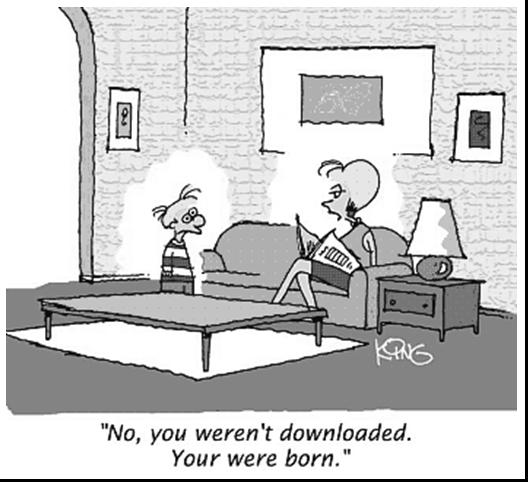
\includegraphics[width=.5\textwidth]{fig1.jpg}
\caption{A typical figure}
\label{fig:exampleFig1}
\end{figure}

\begin{figure}[ht]
\centering
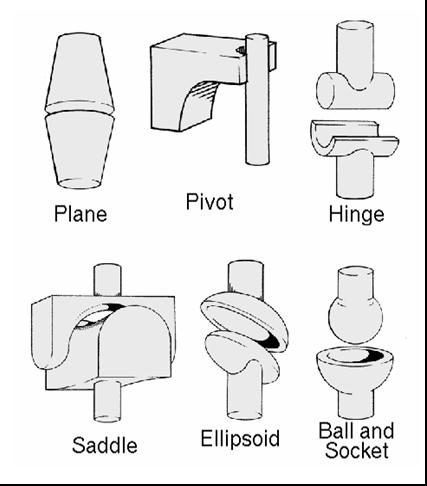
\includegraphics[width=.3\textwidth]{fig2.jpg}
\caption{This figure is an example of a figure caption taking more than one
  line and justified considering margins mentioned in Section~\ref{sec:figs}.}
\label{fig:exampleFig2}
\end{figure}

In tables, try to avoid the use of colored or shaded backgrounds, and avoid
thick, doubled, or unnecessary framing lines. When reporting empirical data,
do not use more decimal digits than warranted by their precision and
reproducibility. Table caption must be placed before the table (see Table 1)
and the font used must also be Helvetica, 10 point, boldface, with 6 points of
space before and after each caption.

\begin{table}[ht]
\centering
\caption{Variables to be considered on the evaluation of interaction
  techniques}
\label{tab:exTable1}
\smallskip
\begin{tabular}{|l|c|c|}
\hline
& Value 1 & Value 2\\[0.5ex]
\hline
&&\\[-2ex]
Case 1 & 1.0 $\pm$ 0.1 & 1.75$\times$10$^{-5}$ $\pm$ 5$\times$10$^{-7}$\\[0.5ex]
\hline
&&\\[-2ex]
Case 2 & 0.003(1) & 100.0\\[0.5ex]
\hline
\end{tabular}
\end{table}

\section{Images}

All images and illustrations should be in black-and-white, or gray tones,
excepting for the papers that will be electronically available (on CD-ROMs,
internet, etc.). The image resolution on paper should be about 600 dpi for
black-and-white images, and 150-300 dpi for grayscale images.  Do not include
images with excessive resolution, as they may take hours to print, without any
visible difference in the result. 

\section{References}
      Hamid F, HyunYong L and Akihiro N, ’Software-Defined Networking: A survey’, Computer Networks, 2015.

      Garzon J, Adamuz-Hinojosa O, Ameigeiras P, ’Handover Implementation in a 5G SDN-based Mobile Network Architecture’, PIMRC: Mobile and Wireless Networks, 2016

\bibliographystyle{sbc}
\bibliography{sbc-template}

\end{document}
